% cv_english.tex
\documentclass[11pt]{article}
\usepackage{style}

\begin{document}

% =============================
% Header
% =============================
\hspace{10pt}
\begin{minipage}[t]{0.7\textwidth}
  \hspace{-35pt}
  {\Huge \MyNameEN}

  \vspace{1em}
  \hspace{-33pt}
  Email:\MyEmail 

  \hspace{-33pt}
	Phone:\MyPhone 

  \hspace{-33pt}
	GitHub:\href{\MyGitHub}{\MyGitHub}

  \hspace{-33pt}
	Website:\href{\MyWebsite}{\MyWebsite}
\end{minipage}
% \begin{minipage}[t]{0.2\textwidth}
%   \vspace{-28pt} % ensures alignment at top
%   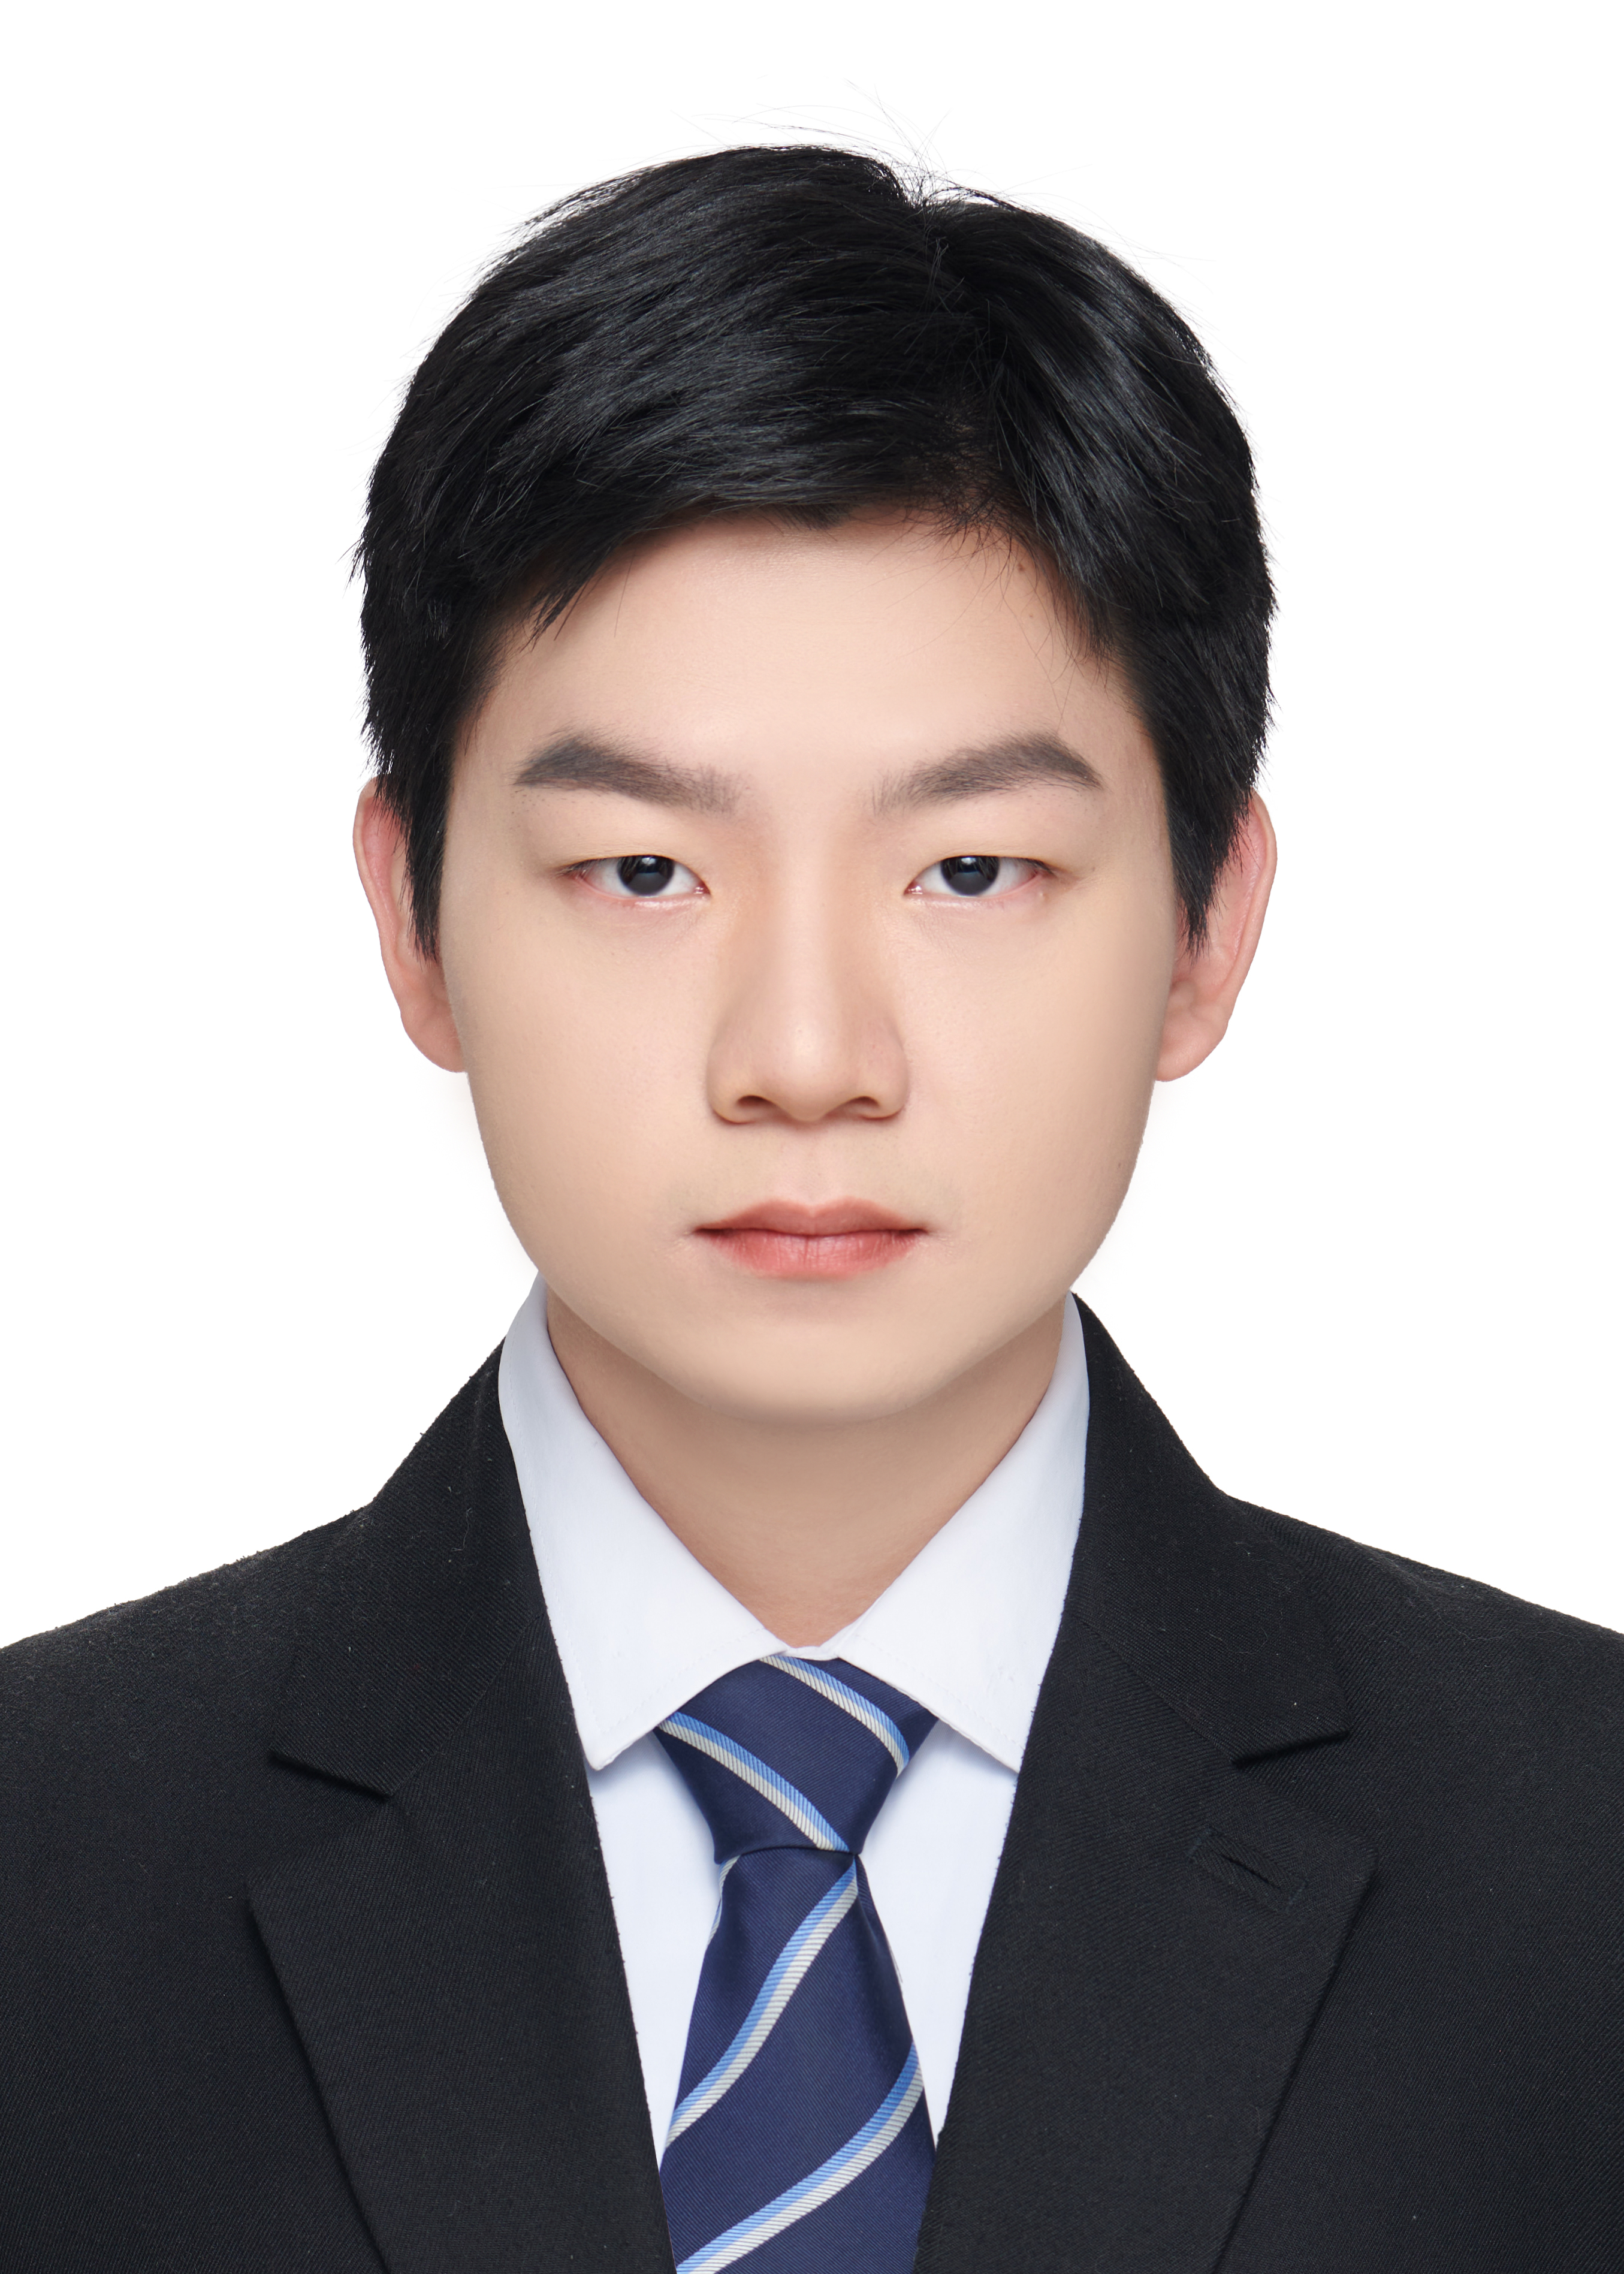
\includegraphics[width=\textwidth]{./images/profile.jpg} 
% \end{minipage}
\hfill

\vspace{1em}


% =============================
% Education
% =============================
\CVSection{Education}
\EducationEntryEN{University of Sydney}{February 2021 -- November 2025}
{Bachelor of Advanced Computing}{Computer Science}

\EducationEntryEN{University of Sydney}{February 2021 -- November 2025}
{Bachelor of Commerce}{Finance}


% =============================
% Publications
% =============================
\CVSection{Publications}
\PublicationEntry{Optimal Look-back Horizon for Time Series Forecasting in Federated Learning}{AAAI 2026 Oral}{\underline{Dahao Tang}, Nan Yang, Yanli Li, Zhiyu Zhu, Zhibo Jin, Dong Yuan}

\PublicationEntry{Stability-Driven CNN Training with Lyapunov-Based Dynamic Learning Rate}{ADC 2024}
{\underline{Dahao Tang}, Nan Yang, Yunkun Deng, Yuning Zhang, Abubakar Sadiq Sani, Dong Yuan }

\PublicationEntry{Adaptformer: An Adaptive Multimodel Deep Decomposition Approach for Power Consumption Forecasting}{ADMA 2024}
{Nan Yang, Yuning Zhang, Yunqi Wang, \underline{Dahao Tang}, Yanli Li, Dong Yuan}


% =============================
% Work Experience
% =============================
\CVSection{Work Experience}
\ExperienceEntryEN{University of Sydney}{August 2024 -- Present}
{Academic Tutor, School of Computer Science}
{\\
ISYS2120 Data and Information Management (2024 S2) \\
}

\ExperienceEntryEN{University of Sydney}{November 2024 -- Present}
{Research Assistant, School of Life and Environment Science}
{Developer of ProteHome at David James Lab}


% =============================
% Projects
% =============================
\CVSection{Projects Experience}
\ExperienceEntryEN{ProteHome}{July 2024 -- Present}
{Research Assistant, Web Development}
{Participated in website refactoring, decided the tech stack of using Next.js, Django, PostgreSQL, Tailwind etc. Continuously Contributed to full-stack development.}

\ExperienceEntryEN{ioulia.ai}{January 2024 -- July 2024}
{Co-founder}
{Designed the technical roadmap, developed the MVP, and optimized product performance using techniques like Chain of Thoughts etc.}

\ExperienceEntryEN{GigHero}{April 2023 -- August 2024}
{Co-founder}
{Developed an MVP platform for an online marketplace for onsite services using React, Express, PostgreSQL, Tailwind etc.}

\ExperienceEntryEN{Searten}{August 2023 -- November 2023}
{University Project, Project Manager, Full-stack Developer}
{Led a team to develop an MVP platform using Next.js and Tailwind etc.}

\ExperienceEntryEN{Student Management Platform}{2022}
{Full-stack Developer}
{Developed a full-stack student management platform using Django.}

\ExperienceEntryEN{File System Implementation with FUSE}{2022}
{University Project}
{Developed a file system in C, supporting large files and directories.}

\ExperienceEntryEN{OS Scheduler Implementation}{2022}
{University Project}
{Designed and implemented an operating system scheduler using Round Robin and MLFQ algorithms in C.}


\end{document}
